\PassOptionsToPackage{unicode=true}{hyperref} % options for packages loaded elsewhere
\PassOptionsToPackage{hyphens}{url}
%
\documentclass[]{article}
\usepackage{lmodern}
\usepackage{amssymb,amsmath}
\usepackage{ifxetex,ifluatex}
\usepackage{fixltx2e} % provides \textsubscript
\ifnum 0\ifxetex 1\fi\ifluatex 1\fi=0 % if pdftex
  \usepackage[T1]{fontenc}
  \usepackage[utf8]{inputenc}
  \usepackage{textcomp} % provides euro and other symbols
\else % if luatex or xelatex
  \usepackage{unicode-math}
  \defaultfontfeatures{Ligatures=TeX,Scale=MatchLowercase}
\fi
% use upquote if available, for straight quotes in verbatim environments
\IfFileExists{upquote.sty}{\usepackage{upquote}}{}
% use microtype if available
\IfFileExists{microtype.sty}{%
\usepackage[]{microtype}
\UseMicrotypeSet[protrusion]{basicmath} % disable protrusion for tt fonts
}{}
\IfFileExists{parskip.sty}{%
\usepackage{parskip}
}{% else
\setlength{\parindent}{0pt}
\setlength{\parskip}{6pt plus 2pt minus 1pt}
}
\usepackage{hyperref}
\hypersetup{
            pdftitle={Intertemporal Choice: A review of the Discount Functions and its implications},
            pdfauthor={Fernando Agustin Falbo*},
            pdfborder={0 0 0},
            breaklinks=true}
\urlstyle{same}  % don't use monospace font for urls
\usepackage[margin=1in]{geometry}
\usepackage{longtable,booktabs}
% Fix footnotes in tables (requires footnote package)
\IfFileExists{footnote.sty}{\usepackage{footnote}\makesavenoteenv{longtable}}{}
\usepackage{graphicx,grffile}
\makeatletter
\def\maxwidth{\ifdim\Gin@nat@width>\linewidth\linewidth\else\Gin@nat@width\fi}
\def\maxheight{\ifdim\Gin@nat@height>\textheight\textheight\else\Gin@nat@height\fi}
\makeatother
% Scale images if necessary, so that they will not overflow the page
% margins by default, and it is still possible to overwrite the defaults
% using explicit options in \includegraphics[width, height, ...]{}
\setkeys{Gin}{width=\maxwidth,height=\maxheight,keepaspectratio}
\setlength{\emergencystretch}{3em}  % prevent overfull lines
\providecommand{\tightlist}{%
  \setlength{\itemsep}{0pt}\setlength{\parskip}{0pt}}
\setcounter{secnumdepth}{5}
% Redefines (sub)paragraphs to behave more like sections
\ifx\paragraph\undefined\else
\let\oldparagraph\paragraph
\renewcommand{\paragraph}[1]{\oldparagraph{#1}\mbox{}}
\fi
\ifx\subparagraph\undefined\else
\let\oldsubparagraph\subparagraph
\renewcommand{\subparagraph}[1]{\oldsubparagraph{#1}\mbox{}}
\fi

% set default figure placement to htbp
\makeatletter
\def\fps@figure{htbp}
\makeatother

\usepackage{floatrow}
\floatsetup[figure]{capposition=top}
\floatsetup[table]{capposition=top}
\usepackage{tikz}
\usepackage{pgfplots}
\usepackage{booktabs}
\usepackage{longtable}
\usepackage{array}
\usepackage{multirow}
\usepackage{wrapfig}
\usepackage{float}
\usepackage{colortbl}
\usepackage{pdflscape}
\usepackage{tabu}
\usepackage{threeparttable}
\usepackage{threeparttablex}
\usepackage[normalem]{ulem}
\usepackage{makecell}
\usepackage{xcolor}

\title{Intertemporal Choice: A review of the Discount Functions and its implications}
\author{Fernando Agustin Falbo*}
\date{May, 2018}

\begin{document}
\maketitle
\begin{abstract}
This work has three main goals. First, review three different discount models: the Exponential Discount Function, The Hyperbolic Discount Function and the Quasi-Hyperbolic Discount Function. The different features of these three models have different implications to deal with anomalies found empirically. Second, show how time inconsistency and decreasing discount rates affect decision making, causing Present Bias and Lack of Self Control. Finally, show how the latter two problems are solved by self mechanisms.
\end{abstract}

\textbf{Keywords: }Behavioral Economics, Discount Functions, Exponential Discount, Hyperbolic Discount, Quasi-hyperbolic discount, Present Bias, Self Control.

\vspace*{3ex}

* \textbf{New York University}

\pagebreak

\hypertarget{introduction}{%
\section{Introduction}\label{introduction}}

In this paper, I will study three different models to explain inter-temporal decision making and discount of future utilities. The traditional Discount Utility Model is based on an exponential discount function, which is very useful to approach several economics problems. However, exponential function is limited and does not capture anomalies observed empirically. This limitation causes the emergence of other discount functions,
such as hyperbolic and quasi-hyperbolic, which contemplate problems related to time consistency.

In the first section, the exponential discount function will be addressed. The main advantages of adopting the exponential function will be explained, as well as the empirically observed anomalies that contrasted with the exponential model.

In sections 2 and 3, hyperbolic function and quasi hyperbolic function will be presented respectively. The main proposed forms will be studied and explained to what extent they could solve two of the main anomalies of the exponential function: the decreasing discount rate and inter-temporal inconsistency.

In section 4, one of the most studied problems in Behavioral Economics will be discussed more deeply: present bias and lack of self-control as consequences of hyperbolic discounting. Additionally, two internal mechanisms will be presented to deal with this problem: sophistication and self bargaining. Finally, the conclusions will be presented.

\hypertarget{exponential-discount}{%
\section{Exponential Discount}\label{exponential-discount}}

\hypertarget{the-model}{%
\subsection{The Model}\label{the-model}}

The lifetime individual utility depends on a sequence of present and future consumptions in different periods. According to the traditional discounted utility theory, this could be represented in the following way:

\[
U = f(c_{o}, c_{1}, c_{2},\dots, c_{\infty})
\]

Where \(U\) is the lifetime utility and \(c_{t}\) is consumption at time \(t\). More specifically, the consumer's decision problem adopts an utility lifetime which depends on the discounted instantaneous utility at each time \(t\).

\[
U = \delta^0 u(c_{0})+ \delta^1 u(c_{1}) + \delta^2 u(c_{2}) + \dots + \delta^\infty u(c_{\infty})
\]

or

\[
U = \sum_{t=0}^{\infty}\delta^t u(c_{t})
\]

All the instantaneous utilities are preceded by a discount function \(F(t) = \delta^t\), where \(\delta \epsilon(0,1)\) is the discount factor. The main reason because future payoffs are discounted is that there is a human tendency to value less the future payoffs than the present ones. Risk and uncertainty are also mentioned as reasons for the presence of a discounting factor.

Note that the individual is impatient when \(\delta<1\) as \(F(t)\) is decreasing, is patient when \(\delta>1\) as \(F(t)\) is increasing, and is indifferent between present and future consumption when \(\delta=1\) as \(F(t)\) is constant.

\begin{figure}

{\centering 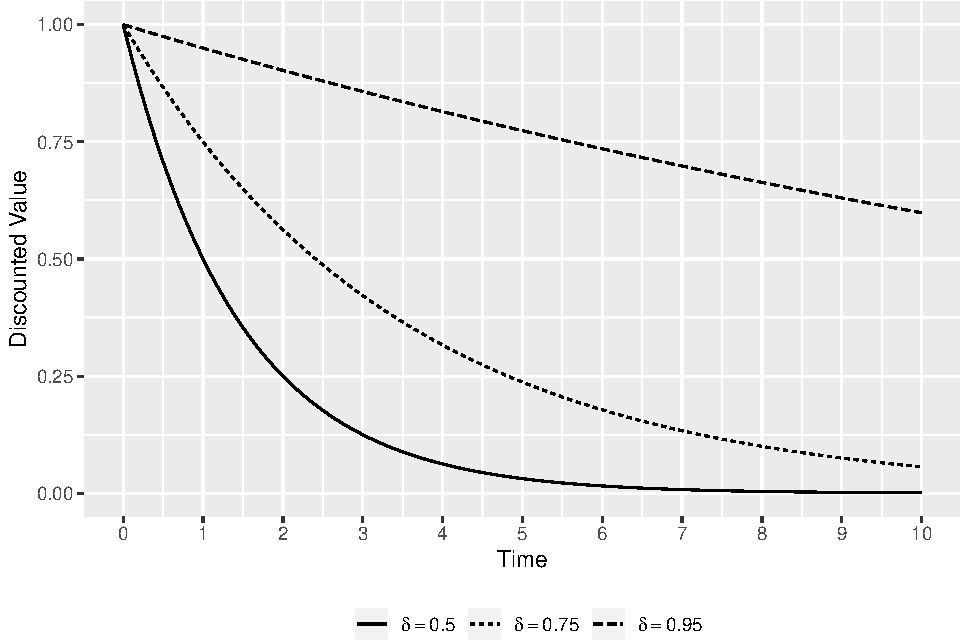
\includegraphics[width=0.75\linewidth]{Discount_Functions_files/figure-latex/exp-1} 

}

\caption{Exponential Discount Functions}\label{fig:exp}
\end{figure}

The value of \(\delta\) depends on the discount rate \(\rho\).

\[
\delta = \frac{1}{1+\rho}
\]

The parameter \(\rho\) represents an individual preference over the future discounting and is constant (does not depend on time). It can be interpreted as the individual 's impatience.

Several exponential discount functions were simulated with different values for \(\delta\). The results are presented in Figure \ref{fig:exp}.

The exponential discount function has two main features, for which it has become very popular in economic models. First, it is ``mathematically nice" since it is additive (Burkett, 2006). This allows to find a solution for \(\delta\) adding infinite series using geometric successions.

\[
1 + \delta + \delta^2 + \dots = \sum_{t=0}^{\infty}\delta^t = \frac{1}{1 - \delta}
\]

The second feature is that it implies inter-temporal consistency. That means the plans settled in one moment are still attractive at all subsequent moments(Burkett, 2006). In ot her words, preferences do not change over time. Given that the discount factor \(\delta\) and the discount rate \(\rho\) are time constant, the preferences are consistent over time. Note that this consistency implies the following: if an individual chooses \$110 tomorrow instead of \$100 today, she will also prefer \$110 in day 31 over \$100 in day 30. In addition to this, the consistency given by the exponential function also ensures that in day 30, she will not change her plan. She will still prefer \$110 the next day (day 31) over \$100 the same day.

\hypertarget{anomalies-in-exponential-discount}{%
\subsection{Anomalies in Exponential Discount}\label{anomalies-in-exponential-discount}}

Read(2007) states seven anomalies of the Exponential model. I will briefly describe them in the following paragraphs. Since I will present the Hyperbolic and the Quasi-hyperbolic models in the following sections, I will focus on the first two anomalies (related with time inconsistency and decreasing discount rates)\footnote{Other anomalies such as Magnitude Effect and Sign Effect are contemplated by other type of functions. Read (2007) presents a \emph{Value Function}, which deals with these kind of problems}.

\begin{itemize}
\tightlist
\item
  \emph{Time Inconsistency}\\

  \begin{itemize}
  \tightlist
  \item
    \emph{Cross-sectional} time inconsistency occurs when people have two different preferences for two different periods. The most popular example is when an individual prefers \$100 today than \$110 tomorrow, but prefers \$110 in 31 days than \$100 in 30 days. As Read (2007) stressed, Kirby and Herrnstein (1995) showed that people choose the small sooner prize over the large prize later for the present, but they change their choice when the same question is asked for a delay in time.\\
  \item
    \emph{Longitudinal} time inconsistency refers to changes in plans because preferences for sooner payoffs increase as they become closer in time. Following the previous example, Fredrick, Loewenstein \& O'Donoghue (2002) shows that in \(t=0\) the subjects chooses to receive \$110 on day 31 (vs \$100 on day 30), but after the 30 days they are asked again and change their mind. After a specified time delay, they prefer \$100 in day 30 over waiting one day for \$110.\\
  \end{itemize}
\item
  \emph{Delay Effect} refers to the existence of decreasing discount rate. Burkett (2006) presents a popular experiment realized by Thaler (1981), where median responses indicated indifference between \$15 today, \$20 in a month, \$50 in a year, and \$100 in ten years. This preferences are in conflict with the exponential discount function, given that they imply different \(\delta\) values for different periods. Indifference between \$15 today and \$50 in one year implies that \(\delta=0.3\), which implies \(\rho=2.3\). On the other hand, indifference between \$15 today and \$20 in a month implies \(\delta=0.0317\), or \(\rho=30.54\). Therefore, \(\delta\) increases in \(t\), while \(\rho\) decreases in \(t\). This means that people are more impatient for immediate payoffs than for future payoffs. The different \(\delta\) and \(\rho\) values corresponding to the example in Burkett (2006) are presented in Table \ref{tab:inc}.\\
\end{itemize}

\begin{table}
    \caption {Inter-Temporal Inconsistent Payoffs} \label{tab:inc}
    \centering
    \begin{tabular}{c c  c c c} 
        & Now   & 1 Month & 1 Year  & 10 Years  \\ 
        \hline 
        $\delta$ &        & $0.0317$  & $0.3$  & $0.8272$  \\ 
        $\rho$   &        & $30.57$   & $2.3$  & $0.209$  \\ 
        Payoff   & \$15   & \$20      & \$50   & \$100  \\ 
        \hline 
    \end{tabular} 
\end{table}

\begin{itemize}
\item
  \emph{Interval Effect} means that the interval between two periods affects the values of \(\delta\) and \(\rho\). Longer intervals lead to smaller discount rates and larger discount factors.\\
\item
  \emph{Direction Effect} refers to the asymmetric preference between delaying and speeding up consumption. Loewenstein (1988) found that \emph{``The value put on a given delay was much greater when the certificate was delayed than when it was expedited."}(Read, 2007).\\
\item
  \emph{Magnitude Effect} means that the discount rate \(\rho\) is higher for smaller amounts. The exponential function assumes that the discount rate is independent of the size or magnitude of payoffs, but empirical evidence suggest that it is not the case. Individuals discount larger payoffs at a lower rate compared to smaller payoffs. Read provides several works where magnitude effects were found: Kirby (1997), Shelley (1993), and Green, Myerson and McFadden (1997).\\
\item
  \emph{Sign Effect} refers to lower discount rates for losses than for gains. Although the exponential model assumes that the discount rate is independent of the sign of payoffs, evidence suggests that individuals are more impatient to gain a positive reward than to postpone a loss. Loewenstein (1988) found that people were indifferent to win \$100 now and \$157 in a year, but they were also indifferent to lose \$100 now and \$133 in the same year, which implied higher rates for positive amounts than for negative amounts.\\
\item
  \emph{Sequence Effect} means that people usually prefer constant or increasing sequences of outcomes than decreasing ones, which is not compatible with the positive rate of time preference in the exponential model. Loewenstein \& Sicherman (1991) showed that most people in their experiment prefer the increasing sequence even though it implied a lower net present value.
\end{itemize}

\hypertarget{hyperbolic-discount}{%
\section{Hyperbolic Discount}\label{hyperbolic-discount}}

Impatience decreasing is not captured by the exponential discount function, so the Hyperbolic discount function must be used to be compatible with a decreasing discount rate \(\rho\). A simple functional form for the discount function \(F(t)\) was suggested by Ainslie (1975):

\[
F(t)= \frac{1}{t}
\]

As time passes, the value of \(F(t)\) falls. This can be shown with

\[
\frac{\partial F(t)}{\partial t}= \frac{-1}{t^2} <0
\]

And

\[
\frac{\partial^2 F(t)}{\partial t^2}= \frac{2}{t^3} > 0
\]

Which is consistent with decreasing impatience.

Another form was proposed by Mazur (1984):

\[
F(t, \rho)= \frac{1}{1 + \rho t}
\]

This specification is better in the sense that it states a relationship between the discount function and the discount rate. It can be shown that when as both \(t\) and \(\rho\) increase, the function value decreases

\[
\frac{\partial F(t, \rho)}{\partial \rho}= \frac{-t}{(1 + \rho t)^2} < 0 
\]

And

\[
\frac{\partial F(t, \rho)}{\partial t} = \frac{-\rho}{(1 + \rho t)^2} < 0 
\]

With

\[
t, \rho > 0
\]

Additionally, it is possible to determine more specifically the decreasing impatient in time:

\[
\frac{d \rho}{d t} = -\frac{F_{t}(t, \rho)}{F_{\rho}(t, \rho)} =  -\frac{t}{\rho} < 0
\]

With

\[
t, \rho > 0
\]

which is also consistent with decreasing impatience.

Ultimately, Loewenstein \& Prelec (1992) present the general case:

\[
F(t)= \frac{1}{(1 + \alpha t)^{\gamma/\alpha}} 
\]

With

\[
\gamma, \alpha > 0
\]

Where \(\alpha\) measures the distance to the exponential discounting and \(\gamma\) represents a time preference parameter. This specification is considered to provide the best fit with experimental data (Streich and Levy, 2007).

From Figure \ref{fig:hyp} it it is possible to see the differences between the exponential and the hyperbolic function. Starting from \(t=0\), the discount function values decreases with time for both specifications. However, exponential discounting implies discount at a constant rate, while hyperbolic discounting implies discount at a (gradually) decreasing rate. This can be seen observing that the hyperbolic function curve is steeper for the first periods (more impatience) and becomes flatter with time (more patience in the future periods), whereas exponential curve's slope decreases smoothly. Actually, after period 7 the Ainslie and Loewenstein functions show greater values than the exponential function. Read (2007) refers to the point where the utilities curves cross each other as \emph{Indifference point / Preference reversal}.

\begin{figure}

{\centering 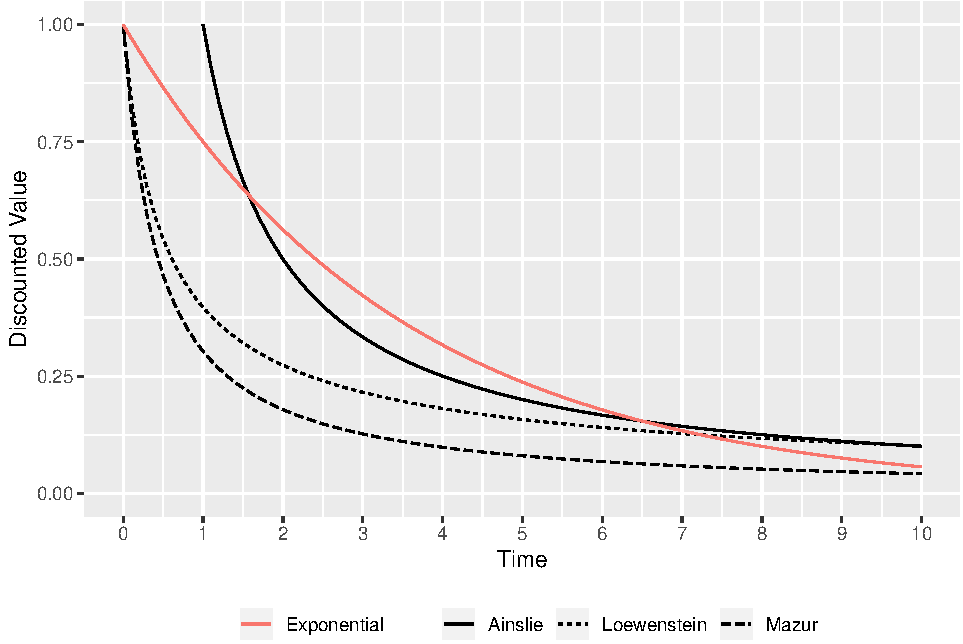
\includegraphics[width=0.75\linewidth]{Discount_Functions_files/figure-latex/hyp-1} 

}

\caption{Hyperolic Discount Functions}\label{fig:hyp}
\end{figure}

\begin{itemize}
\tightlist
\item
  Ainslie: \(\frac{1}{t}\)
\item
  Mazur: \(\frac{1}{(1+ \rho t)}\) with \(\rho = 2.3\)
\item
  Loewenstein: \(\frac{1}{(1+ \alpha t)^(\frac{\gamma}{\alpha})}\) with \(\alpha = 3\) and \(\gamma = 2\)
\item
  Exponential: \(\delta^t\) with \(\delta = 0.75\)
\end{itemize}

The hyperbolic Discount function works to show that the discount rate decreases in the long term, but it also requires a sort of consistency over time: longitudinal consistency. Back to our example, an individual could choose \$100 today (instead of \$110 tomorrow) and \$110 in 31 days (instead of \$100 in 30 days). This is captured by the hyperbolic discounting, because in \(t=0\) the individual is more patient after 30 days than today. However, if she changes her mind -if she is asked in 30 days and prefers the \$100 in that moment instead to wait one more day to get \$110-, the hyperbolic discount cannot capture this behavior. In other words, hyperbolic discounting can deal with the \emph{delay effect}, but it does not contemplate cases with \emph{longitudinal} time inconsistency.

Regarding to this point, it is necessary to explain in more detail the \emph{Cross-sectional} time consistency -associated with \emph{Date-Independence}- and \emph{longitudinal} time consistency -associated with \emph{Date-Dependence}-. According to Read (2007), date-independence implies that agents not only make consistent plans, but they will also use the same pattern to state plans in every period. This is called cross-sectional time consistency and it would be the case of the exponential discount function. By contrary, with date-dependence agents are allowed to have different discount rates for different periods, but once they stick to a plan, they will not change it. In this case, even though cross-sectional time consistency is violated, longitudinal time consistency holds. \emph{``As has been discussed previously, cross-sectional, but not longitudinal, inconsistencies can occur if the discount rate depends on calendar time rather than temporal distance to the events in question"} (Read, 2012).

This result could be interpreted as following: hyperbolic function allows that the agent becomes more patient with age. In the \$100 vs \$110 example, the future older agent (thirty days from now) will be more patient than the present younger agent, but the hyperbolic function is still in conflict when the agent is more impatient for short term gains than for long term gains at any period.

Therefore, another function is needed to explain the cases when people make a plan, but then they change it.

\hypertarget{quasi-hyperbolic-discount}{%
\section{Quasi-Hyperbolic Discount}\label{quasi-hyperbolic-discount}}

Quasi-Hyperbolic Discount Function is useful to deal not only with different discount-rates over time, but also with \emph{preference reversal}. The conceptual distinction with the hyperbolic function is that time period should not be interpreted as a specific date, but as reference to start counting discount factors \footnote{Note that Rasmusen (2008) considers this feature to all non-exponential functions (which he calls hyperbolic functions). In this work, I followed Cartwright (2011), where time as specific dates is used in exponential and hyperbolic function and time as a delay reference is used in quasi-hyperbolic function.}. In this way, the economic agent is always more impatient for short term gains, since in the following periods the initial discount factors chain starts again and again.

Read (2012) stresses that the two models differ in:

\begin{itemize}
\tightlist
\item
  In the hyperbolic model discount rate decreases with time gradually, while in the quasi-hyperbolic model \emph{``there is a threshold delay which leads to excess discounting, after which there is constant rate discounting thereafter''} (Read, 2012).
\item
  Hyperbolic discounting implies that the discount rate will be reduced to almost zero in the long run, whereas quasi-hyperbolic discounting assumes a constant discount rate for all delays \emph{``once the initial delay is past, so even a small discount rate can lead even large outcomes to have zero value which entails disregard for the distant future''} (Read, 2012).
\end{itemize}

Phelps \& Pollak (1968) proposed the form:

\[
U = \delta^0 u(c_{0})+ \beta\delta^1 u(c_{1}) + \beta\delta^2 u(c_{2}) + \beta\dots + \beta\delta^\infty u(c_{\infty}) 
\]

With \(0<\beta, \delta <1\)

or

\[
U = u(c_{0})+ \beta \sum_{t=1}^{\infty}\delta^{t} u(c_{t})
\]

Note that if \(\beta=1\), this form is the exponential function. The difference here is that since \(0<\beta<1\), utility today is even more valued than utility in the future. In other words, besides the obvious discount function \(F(t)=\delta^t\) (which is decreasing in \(t\)), there is an ``additional'' discount factor \(\beta\), which makes the present utility more valuable. Therefore, \(\beta\) reflects the presence of a sort of ``myopia''.

If \(\beta\) is close to \(0\), then the individual is extremely impatient in the present. \(\beta\) can be also interpreted as a measure of \emph{present bias}. Note that the quasi-hyperbolic function contemplates the cases where the agents make a plan and then change it. In the previous example of choosing \$100 today (vs \$110 tomorrow) and \$100 in 30 days (vs \$110 in 31 days), the chain of discount factors faced by the agent will be the same in both cases (today and in 30 days). Therefore, at day 30 the present bias will appear again because the discount factor for the future will be the same than in day 1, so she will choose to get \$100 in that moment instead of wait one more day to get \$110.

Another popular specification for quasi-hyperbolic function is given by Laibson (1997):

\[ F(t)=\begin{cases} 
1 & t = 0 \\
\beta\delta^t & t>0 \\ 
\end{cases}
\]

Based on empirical evidence, Laibson (1997) further suggests that \(\beta\) should be calibrated in the interval \((0, 2/3 )\) assuming that \(\delta\) is close to unit. In Figure \ref{fig:qh}, Laibson quasi-hyperbolic specification simulations are presented with \(\beta=0.75\) and \(\beta=0.95\) for \(\rho=0.95\). Additionally, hyperbolic function and exponential function can be seen to compare the three cases.

\begin{figure}

{\centering 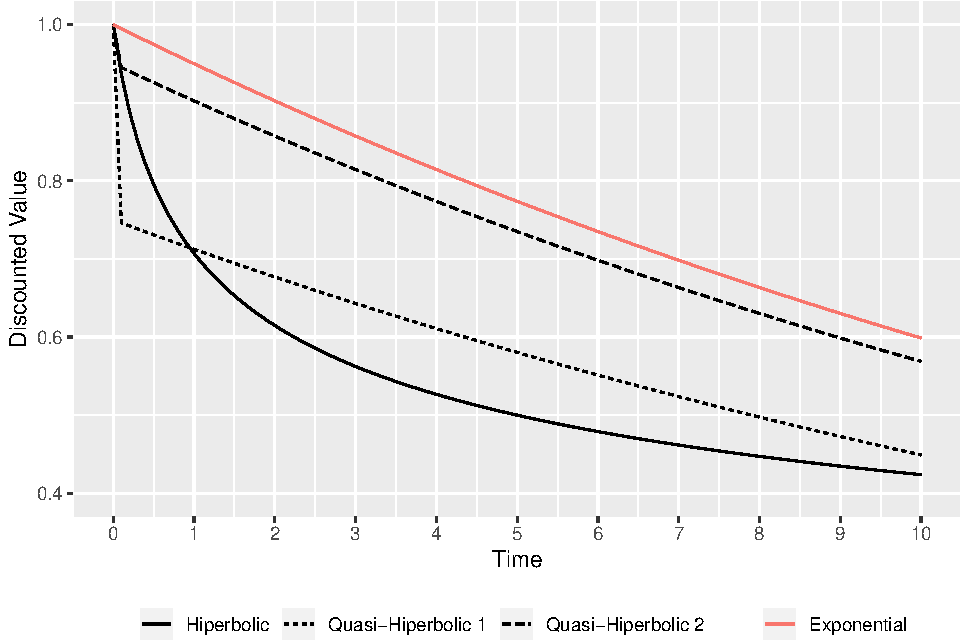
\includegraphics[width=0.75\linewidth]{Discount_Functions_files/figure-latex/qh-1} 

}

\caption{Quasi-Hyperbolic Discount Functions}\label{fig:qh}
\end{figure}

\begin{itemize}
\tightlist
\item
  Quasi-Hyperbolic 1: \(\beta = 0.75\), \(\delta = 0.95\)
\item
  Quasi-Hyperbolic 2: \(\beta = 0.95\), \(\delta = 0.95\)
\item
  Hyperbolic: \(\alpha = 3\), \(\gamma = 1\)
\item
  Exponential: \(\delta = 0.95\)
\end{itemize}

The characteristics commented above are shown in Figure \ref{fig:qh}. The quasi-hyperbolic function shows a discount rate decreasing very fast (steeper slope) at the beginning, but after a threshold it is very similar to the exponential function with constant decreasing rate. On the other hand, the discount rate decreases faster at beginning (not so fast as the quasi-hyperbolic function value) and gradually with time for the hyperbolic function.

A briefly resume of the three discount models seen above is presented in Table \ref{tab:dis}.

\begin{table}
    \caption {Discount Models} \label{tab:dis}
    \centering
    \begin{tabular}{l c c c c}
        \hline
                          & Exponential                    & Hyperbolic*                         & Quasi-Hyperbolic \\ 
        \hline
        Discount Function & $F(t)= \delta^t$               & $F(t, \rho)= \frac{1}{1 + \rho t}$  & $F(t)=\beta \delta^t$ \\ 
        Discount Rate     & $\rho=\frac{1-\delta}{\delta}$ & $\rho=\frac{1-\delta}{\delta t}$    & $\rho=\frac{1-\delta}{\delta}$ \\ 
        Time              & Specific Date                  & Specific date                       & Reference/Delay  \\ 
        Cross-Sectional Inconsistency & X                  & $\surd$                             & $\surd$ \\ 
        Longitudinal Inconsistency    & X                  & X                                   & $\surd$ \\ 
        Delay Effect                  & X                  & $\surd$                             & $\surd$ \\ 
        \hline
        \begin{minipage}{0.2\textwidth}
            {\footnotesize * Mazur, 1984}
        \end{minipage}
    \end{tabular}
\end{table}

\hypertarget{lack-of-self-control-and-how-to-deal-with-it}{%
\section{Lack of Self-Control and how to deal with it}\label{lack-of-self-control-and-how-to-deal-with-it}}

It has been shown that time inconsistency and decreasing discount rate are anomalies in the exponential function. Therefore, hyperbolic and quasi-hyperbolic functions were introduced and explained to deal with these problems. The question arising now is: What are the implications of these anomalies? What does it mean that people cannot stick to a plan? How they deal with these problems when they have to make decisions?

In this section, I will focus on one of the most important consequences of the temporal inconsistency: the lack of self-control to make decisions. The fact that people have a lower rate of impatience in the present than in the future, that is to say, that they suffer of present bias, means that they cannot stick to their plans.
Two of the most used examples to reflect the problem of self-control are those of the smoker and the individual who wants start a diet-regime. Both the smoker and the overweight person suffer from lack of self control when they decide to stop smoking / eat healthy in the future but can never achieve it. In the previous sections I explained the presence of present bias from a formal perspective. Now, I will explain how this affect decision making from the conceptual perspective, using the examples of the smoker and the overweight person.

For the future, they vow to quit smoke and unhealthy food in exchange for long term rewards (better health) because they use a smaller discount rate for rewards in the future. However, as times go by, the pleasure of smoking a cigarette or eating cake are very high. Therefore, the smoker and the overweight individual decide to smoke a cigarette and eat a cake today, but plan to stop doing so next month. When the next month arrives, the present bias comes back into action, because the option of smoking and eating unhealthy are again very desirable, since the pleasure of doing so now is very high. This problem of self-control produces that the individuals cannot respect their plans and leave unhealthy habits becomes very difficult.

Several authors from Behavioral Economics proposed different mechanism to fix the problem of self control. Different kinds of \emph{Paternalism} were discussed in the last decades. Explain how Paternalism deal with present bias and lack of self control is not part of this paper. However, it is interesting to know that there are other ``self-mechanisms" (often used against Paternalism proposals) to deal with these problems. In the following paragraphs I will briefly describe \emph{internalities and self-bargaining} and \emph{sophistication}.

\hypertarget{internalitites-and-self-bargaining}{%
\subsection{Internalitites and Self Bargaining}\label{internalitites-and-self-bargaining}}

Another way of thinking about this problem is within the framework of \emph{internalities}. Whitman (2006) explains how internalities give place to \emph{self-bargaining} and a consistent result.
If we split an individual into two selfs, we can define the present-self and the future-self. The present-self wants to smoke because she perceives the pleasure of smoking, while the future-self does not want the individual-self to smoke, since it has negative consequences for her health. This is based on the idea that externalities are reciprocal: if the present-self smokes, it has a negative effect on the future-self, but if the present-self does not smoke, it has a negative effect on herself. These externalities between different selfs in the time of a single individual are called internalities. Can this internality be solved?

A bargaining between the present-self and a representation of the future-self in the present is necessary. If the contract is very strict and rigid (smoking is not allowed), it is very likely that the present-self does not respect the contract and all benefits will be lost. If, on the other hand, the contract allows exceptions (such as smoking less quantity or having certain foods allowed on some occasions), it is more likely that the present-self respect the contract.

Note that a plan like this is consistent in time. The individual has a contract with her future-self, which specifies the special situations when she is able to eat something not allowed in the regular diet or smoke a cigar.

\hypertarget{sophistication}{%
\subsection{Sophistication}\label{sophistication}}

In the following paragraphs I will follow the examples of Cartwright (2011) to explain \emph{sophistication}, another internal tool to deal with present bias. Suppose on Friday, Maria must decide when she will do her homework (to be submitted on Monday). If Maria does not have present bias (\(\beta = 1\)), on Friday the best plan is to do the homework on Saturday, since it has the highest payoff (10.9). On Saturday, doing homework on Saturday is still the best plan, because Maria keep getting the highest payment (in this case 12.1). Something similar happens when Maria has just a little bit of present bias (\(\beta = 0.9\)). The plan to do homework on Saturday is better on both Friday and Saturday. Therefore Maria does the homework on Saturday and there are no major problems.

However, when Maria has greater present bias (\(\beta = 0.8\)) the problem becomes more complex. On Friday, Maria plans to do her homework on Saturday because she gets the highest payment (8.7), but on Saturday, the present bias comes into action and higher discount for nearest future makes the payment of doing homework on Monday (9.0) greater than doing it on Saturday (8.7). In this way, a reversion of the preferences is observed.

\begin{table}

\caption{\label{tab:s1}Homework: Costs First}
\centering
\begin{tabular}[t]{lcccc}
\toprule
\multicolumn{1}{c}{} & \multicolumn{1}{c}{On Friday} & \multicolumn{1}{c}{On Saturday} & \multicolumn{1}{c}{On Friday} & \multicolumn{1}{c}{On Saturday} \\
\cmidrule(l{3pt}r{3pt}){2-2} \cmidrule(l{3pt}r{3pt}){3-3} \cmidrule(l{3pt}r{3pt}){4-4} \cmidrule(l{3pt}r{3pt}){5-5}
Plan & $\beta = 1$ & $\gamma = 0.9$ & $\beta= 0.8$ & $\gamma = 0.9$\\
\midrule
Do it Friday & \textcolor{black}{10.5} & \textcolor{black}{-} & \textcolor{black}{7.4} & \textcolor{black}{-}\\
Do it Saturday & \textcolor{blue}{10.9} & \textcolor{blue}{12.1} & \textcolor{blue}{8.7} & \textcolor{black}{8.7}\\
Do it Sunday & \textcolor{black}{7.7} & \textcolor{black}{8.6} & \textcolor{black}{6.2} & \textcolor{black}{7.9}\\
Do it Monday & \textcolor{black}{9} & \textcolor{black}{10} & \textcolor{black}{7.2} & \textcolor{blue}{9}\\
\bottomrule
\end{tabular}
\end{table}

This problem can have two outcomes. The first is that Maria is a \emph{naive} person and does not know that she has present bias. This is a case of \emph{procrastination} and Maria will do the homework on Monday, that is, modify her plan and delay the homework until last moment. The second case is when Maria is \emph{sophisticated} and she is aware of her present bias. In this way, Maria knows that if she waits until Saturday, she will do the homework on Monday. Therefore, the real options are doing the homework on Monday with a payment of 7.2 or doing the homework on Friday with a payment of 7.4, which will lead her to do the homework on Friday and procrastination is avoided. Results for this example are presented in Table \ref{tab:s1}.

In the previous example, costs come before benefits, but the opposing order could lead to different outcomes. Suppose now that Maria must choose which day go to the cinema theater as in Table \ref{tab:s2}. With no present bias, she will plan to go on Sunday and she will stick to her plan. In case of present bias (\(\beta = 0.8\)), on Friday she plans to go on Sunday, since she gets the highest payment (6.5). However, on Saturday she prefers to go on Saturday because she has a higher payment than on Sunday. Again, the outcome will depend on whether Maria is naive or sophisticated. If she is naive, she will end up going to the movies on Saturday. If she is sophisticated, she will go on Friday, that is, she will anticipate her future present bias. In the latter case, we can say that Maria will \emph{preproperate}.

\begin{table}

\caption{\label{tab:s2}Movies: Benefits First}
\centering
\begin{tabular}[t]{lcccc}
\toprule
\multicolumn{1}{c}{} & \multicolumn{1}{c}{On Friday} & \multicolumn{1}{c}{On Saturday} & \multicolumn{1}{c}{On Friday} & \multicolumn{1}{c}{On Saturday} \\
\cmidrule(l{3pt}r{3pt}){2-2} \cmidrule(l{3pt}r{3pt}){3-3} \cmidrule(l{3pt}r{3pt}){4-4} \cmidrule(l{3pt}r{3pt}){5-5}
Plan & $\beta = 1$ & $\gamma = 0.9$ & $\beta= 0.8$ & $\gamma = 0.9$\\
\midrule
Go on Friday & \textcolor{black}{5} & \textcolor{black}{-} & \textcolor{black}{5} & \textcolor{black}{-}\\
Go on Saturday & \textcolor{black}{5.4} & \textcolor{black}{6} & \textcolor{black}{4.3} & \textcolor{blue}{6}\\
Go on Sunday & \textcolor{blue}{6.5} & \textcolor{blue}{7.2} & \textcolor{blue}{5.2} & \textcolor{black}{5.8}\\
\bottomrule
\end{tabular}
\end{table}

Finally, there are other mechanisms to deal with present bias, such as \emph{commitment}. In the movies example, a commitment will imply find someway to force the plan. Particularly, if Maria is sophisticated, on Friday she can buy tickets to go to the movies on Sunday.

\hypertarget{conclusions}{%
\section{Conclusions}\label{conclusions}}

This work showed how the exponential discount function was very useful to build economic models due to its mathematical features and its inter-temporal consistency. However, the empirical evidence shows many anomalies that the exponential function cannot explain.

The hyperbolic and quasi-hyperbolic functions have the advantage that they can deal with problems of decreasing discount rate and inter-temporal inconsistencies, even though they do not contemplate other important anomalies either.

It was also analyzed how the present bias is originated by the hyperbolic / quasi-hyperbolic discount and how it impacts in the decision making process and in the lack of self control. This causes a great difficulty to understand and interpret inter-temporal preferences, and also reveals that individuals are systematically not consistent when it comes to stick to a plan.
Finally, sophistication and self-bargaining were analyzed as mechanisms that can solve, at least partially, the problem of consistency and lack of self-control without the need for superior intervention (paternalism).

\hypertarget{bibliography}{%
\section{Bibliography}\label{bibliography}}

\begin{itemize}
\item
  Ainslie, G. (1975). ``Specious Reward: A Behavioral Theory of Impulsiveness and Impulse Control". Psychological Bulletin, 82(4), 463--96.
\item
  Burkett, J.P. (2006). ``Microeconomics : Optimization, Experiments, and Behavior". Oxford University Press
\item
  Cartwright, E. (2011). ``Behavioral economics". Routledge.
\item
  Fredrick, S., Loewenstein, G. and and O'Donoghue, T. (2002). ``Time Discounting and Time Preference: A Critical Review". Journal of Economic Literature, 40(2), 351--401.
\item
  Kirby, K.N. and Herrnstein, R.J. (1995). ``Preference Reversals Due to Myopic Discounting of Delayed Reward". Psychological Science, 6(2), 83-9.
\item
  Laibson, D. (1997). ``Golden eggs and hyperbolic discounting". The Quarterly Journal of Economics, 112(2), 443--77.
\item
  Loewenstein, G. (1988). ``The Weighting of Waiting: Response Mode Effects in Intertemporal Choice". Working Paper, Center for Decision Research, University of Chicago.
\item
  Loewenstein, G. and Sicherman, N. (1991). ``Do Workers Prefer Increasing Wage Profiles?". Journal of Labor Economics, 9(1), 67--84.
\item
  Loewenstein, G. and Prelec, D. (1992). ``Anomalies in Intertemporal Choice: Evidence and an Interpretation", The Quarterly Journal of Economics, 107(2), 573--97.
\item
  Mazur, J.E. (1984). ``Tests of an equivalence rule for fixed and variable delays". Journal of Experimental Psychology: Animal Behavior Processes, 10, 426-36.
\item
  Phelps, E.S. and Pollak, R. (1968): ``On Second-Best National Saving and Game-Equilibrium Growth". The Review of Economic Studies, 35(2), 185--99.
\item
  Rasmusen, E. (2008). ``Some Common Confusions about Hyperbolic Discounting". Available online at \url{http://www.rasmusen.org/special/hyperbolic-rasmusen.pdf}
\item
  Read, D., Frederick S. and Airoldi, M. (2012). ``Four Days Later in Cincinnati: Longitudinal Tests of Hyperbolic Discounting". Acta Psychologica, vol.~140, pp.177-185.
\item
  Read, D. (2007).``Intertemporal Choice". Blackwell Handbook of Judgment and Decision Making (ed. Derek Koehler and Nigel Harvey), pp.~424-433.
\item
  Streich, P. and Levy, J.S. (2007). ``Time Horizons, Discounting, and Intertemporal Choice". Journal of Conflict Resolution, 51(2), 199--226.
\item
  Thaler, R. (1981). ``Some empirical evidence of dynamic inconsistency". Economics Letters, 8, 201-7.
\item
  Whitman, G. (2006). ``Against the New Paternalism: Internalities and the Economics of Self-Control". Cato Policy Analysis, no. 563.
\end{itemize}

\end{document}
